%&"../ml"
\begin{document}
    \title{第一次作业}
    \maketitle
    
    \section{k-mean 算法}

    \begin{proof}
        对两步分别证明。

        \begin{enumerate}[(a)]
            \item \textbf{E 步} 如果将每一个点 $x_n$ 赋予类 $k_n^\prime$ 使得其相对于其他所有的类最近,即
            \begin{equation*}
                \| x_n-\mu_{k_n^\prime} \| = \min_k{\| x_n - \mu_k\|}
            \end{equation*}
            就意味着它将比上一次赋予的类 $k_n$ 在现在的这种聚类分布下距离不会增加:
            \begin{equation*}
                \| x_n-\mu_{k_n^\prime} \| \leq \| x_n-\mu_{k_n} \|
            \end{equation*}
            那么在对这个点求和的时候,根据指示函数 $r_{nk}$ 的定义,该项也不会增加:
            \begin{equation*}
                j_n = \sum_{k=1}^K r_{nk}^{\prime}\| x_n - \mu_k \|^2 \leq \sum_{k=1}^K r_{nk}\| x_n - \mu_k \|^2
            \end{equation*}
            这里
            \begin{equation*}
                r_{nk} = \begin{cases}
                    1, & \text{$x_n$ 属于类 $k$;}\\
                    0, & \text{其他情况.}
                \end{cases}
            \end{equation*}
            那么损失函数也不会增加:
            \begin{equation}
                J(\mu_1,\cdots,\mu_K) = \sum_{n=1}^N j_n
            \end{equation}
            \item \textbf{M 步} 
            记每个聚类 $k$ 内的点损失函数贡献值为
            \begin{equation}\label{eq:cluster}
                j_k = \sum_{n=1}^N r_{nk}\|x_n-\mu_k\|^2
            \end{equation}
            求和可以交换,损失函数改写为
            \begin{equation}\label{eq:loss}
                J(\mu_1,\cdots,\mu_K)=\sum_{k=1}^K j_k
            \end{equation}
            将用引理 \ref{lem:sqr} 证明,使用聚类内点的平均点作为新的聚类点将不会增加该项。
            \begin{lemma}[距离平方和最小]\label{lem:sqr}
                当 $\mu$ 是所有数据点的均值时,距离平方和
                \begin{equation}\label{eq:dist}
                    f = \sum_{t=1}^N \| \mu-x_t \|^2
                \end{equation}
                最小。
                \begin{proof}
                    将公式 \eqref{eq:dist} 改写
                    \begin{align*}
                        f &= \sum_{t=1}^N \| \mu-x_t \|^2 \\
                          &= \sum_{t=1}^N (\mu-x_t)^T(\mu-x_t) \\
                          &= \sum_{t=1}^N \left(\mu^T\mu - 2x_t^T\mu+x_t^Tx_t\right)
                    \end{align*}
                    对其求导,
                    \begin{align}
                        \frac{\partial f}{\partial \mu} = \sum_{t=1}^N(2\mu^T-2x_t^T)&=0\nonumber\\
                        \mu=\frac{1}{N}\sum_{t=1}^N x_t\label{eq:mean}
                    \end{align}
                    公式 \eqref{eq:mean} 表明当 $\mu$ 是所有数据点的均值时,导数为 0,距离平方和最小。
                \end{proof}
            \end{lemma}
            由于对于每一类而言,公式 \eqref{eq:cluster} 都不会增加,而类别指示函数 $r_{nk}$ 不会改变,所以损失函数 \eqref{eq:loss} 不会增加。
        \end{enumerate}
    \end{proof}

    \section{k-mean 与 GMM 之间}

    \begin{solution}
        为了将 GMM 退化为 k-mean,需要对 GMM 有三个方面的特殊化处理:
        \begin{align}
            \pi_k &= \frac{1}{K} \label{eq:mixing}\\
            \bm{\Sigma} &= \bm{I} \label{eq:conv} \\
            p(k|x_n) &= \begin{cases}
                1, & \text{如果 }k=\arg\max_k\mathcal{N}(x_n|\mu_k,\Sigma_k) \\
                0, & \text{其他情况.}
            \end{cases} \label{eq:oneink}
        \end{align}
        公式 \eqref{eq:mixing} 是混合权重的归一,公式 \eqref{eq:conv} 是协方差一致使得其只计算欧氏距离,公式 \eqref{eq:oneink} 是硬赋值只取可能性最大的那个聚类 $k$。

        为了得到其中一个中间变种,这里我们只退化 \eqref{eq:mixing},使 GMM 中的 $\pi_k=\frac{1}{K}$,就可以得到一个更加一般的带方差项软赋值的 k-mean 算法 \ref{alg:vark}。此时的对数似然值定义为
        \begin{equation}\label{eq:loglike}
            \ln p(\bm{X}|\bm{\mu},\bm{\Sigma})=\sum_{n=1}^N\left[-\ln K + \ln\sum_{k=1}^K\mathcal{N}(\bm{x}_n|\bm{\mu}_k,\bm{\Sigma}_k)\right]
        \end{equation}

        \textbf{优点} 这种算法可以很好地拓展 k-mean 算法,使其能够具有方差项(引入高斯分布),并且软赋值可以更好地考虑多个聚类。
        
        \textbf{缺点} 这种算法无疑增加了一定的计算量。
    \end{solution}

    \begin{algorithm}
        \caption{含方差软赋值的 k-mean 算法}\label{alg:vark}
        \KwIn{数据点 $\bm{X}=\{\bm{x}_n\}_{n=1}^N$, 聚类数目 $K$}
        \KwOut{聚类的分类结果 $\bm{\mu}_j,\bm{\Sigma}_j,\quad\forall j\in \mathbb{N}\cap[1,K]$}
        \BlankLine
        初始化均值矩阵 $\bm{\mu}_k$,协方差矩阵 $\bm{\Sigma}_k$,根据公式 \eqref{eq:loglike} 初始化对数似然值\;
        \Repeat{公式 \eqref{eq:loglike} 中的值没有明显变化}{
            \For{$n\leftarrow 1$ to $N$}{
                \For{$k\leftarrow 1$ to $K$}{
                    \begin{equation}
                        \gamma_{nk}^{(t)}\leftarrow \frac{\mathcal{N}(\bm{x}_n|\bm{\mu}_k,\bm{\Sigma}_k)}{\sum_{j=1}^K\mathcal{N}(\bm{x}_n|\bm{\mu}_j,\bm{\Sigma}_j)}
                    \end{equation}
                }
            }
            \For{$k\leftarrow 1$ to $K$}{
                \begin{align}
                    \bm{\mu}_k^{(t+1)}&\leftarrow\frac{\sum_{n=1}^N\gamma_{nk}^{(t)}\bm{x}_n}{\sum_{n=1}^N\gamma_{nk}}\\
                    \bm{\Sigma}_k^{(t+1)}&\leftarrow\frac{\sum_{n=1}^N\gamma_{nk}^{(t)}(\bm{x}_n-\bm{\mu}_k^{(t+1)})(\bm{x}_n-\bm{\mu}_k^{(t+1)})^T}{\sum_{n=1}^N\gamma_{nk}}
                \end{align}
            }
        }
        \Return{$\bm{\mu},\bm{\Sigma}$}
    \end{algorithm}

    \section{k-mean 与 CL}
        \subsection{k-mean 与 CL 的比较}\label{sec:cl}
        
        见表 \ref{tab:comp}。
        以及,如果将 k-mean 按照 CL 的方法以在线版本的视角去看,可以看到两者在公式上的联系。

        对于一个聚类 $k$ 的前 $N$ 个数据点,获得该聚类的均值点
        \begin{equation}
            \mu^{(N)}_k=\frac{1}{N}\sum_{n=1}^Nx_n
        \end{equation}
        如果该聚类在下一轮后多了一个点,那么更新该聚类的均值点后
        \begin{align}
            \mu^{(N+1)}_k&=\frac{1}{N+1}\sum_{n=1}^{N+1}x_n \nonumber\\
            &=\frac{1}{N+1}\left(N\mu^{(N)}_k+x_{N+1}\right)\nonumber\\
            &=\mu^{(N)}_k+\frac{1}{N+1}\left(x_{N+1}-\mu^{(N)}_k\right)\label{eq:kmean}
        \end{align}
        对比与 CL 的更新公式
        \begin{equation}
            \mu^{(N+1)}_k = \mu^{(N)}_k + \eta p_{k,n}\left(x_{N+1}-\mu^{(N)}_k\right)\label{eq:cl}
        \end{equation}
        这里
        \begin{equation}
            p_{k,n}=\begin{cases}
                1, & \text{如果 }k=\arg\min_j\|x_n-\mu_k\|^2\\
                0, & \text{其他情况}.
            \end{cases}\label{eq:clcond}
        \end{equation}
        可见公式 \eqref{eq:kmean} 是公式 \eqref{eq:cl} 在 $\eta=\frac{1}{N+1}$ 和该点被选中时 $p_{k,n}=1$ 的特殊情形。

        \begin{table}
            \centering
            \caption{k-mean 与 CL 的比较}\label{tab:comp}
            \begin{tabular}{>{\bfseries}lcc}
                \toprule
                   & k-mean & CL \\
                \midrule
                算法类型 & 批学习算法 & 在线学习算法 \\
                超参数 & 不需要 & 需要学习率 $\eta$ \\
                更新方法 & 每次需要遍历 & 每次只更新一个点 \\
                复杂度 & 高 & 相对低 \\
                \midrule
                聚类数目 & \multicolumn{2}{c}{无法决定} \\
                初始化 & \multicolumn{2}{c}{收敛速度依赖初始化} \\
                \bottomrule
            \end{tabular}
        \end{table}

        \subsection{RPCL 版本的 k-mean} 

        RPCL 改变了公式 \eqref{eq:clcond} 使其疏远竞争点
        \begin{equation}
            p_{k,n}=\begin{cases}
                1, & \text{如果 }k=c=\arg\min_j\|x_n-\mu_k\|^2\\
                -\gamma, & \text{如果 }k=r=\arg\min_{j\neq c}\|x_n-\mu_k\|^2\\
                0, & \text{其他情况}.
            \end{cases}\label{eq:rpcl}
        \end{equation}
        这里 $\gamma$ 为可变参量,一般范围是 $[0.05,0.1]$。

        在第 \ref{sec:cl} 节我们了解到 k-mean 是 CL 的一个特殊情形,为了将 RPCL 适配 k-mean,将公式 \eqref{eq:rpcl} 适配进去,得到算法 \ref{alg:rpclk}。这个算法每次会进行批量运算,但会增加移开竞争对手的这个过程。

        \begin{algorithm}
            \caption{RPCL 版本的 k-mean 算法}\label{alg:rpclk}
            \KwIn{数据点 $\bm{X}=\{x_n\}_{n=1}^N$,最大聚类数目 $K$,疏远参量 $\gamma$}
            \KwOut{聚类的分类结果 $\bm{\mu}_j,\quad\forall j\in\mathbb{N}\cap[1,K]$}
            \BlankLine
            初始化均值 $\bm{\mu}_k$,学习率 $\eta=0.01K$\;
            \Repeat{$\bm{\mu}_k$没有明显变化}{
                \For{$n\leftarrow 1$ to $N$}{
                    计算到每个聚类的距离$\bm{E}=\{\|\bm{x}_n-\bm{\mu}_k\|\}_{k=1}^K$\;
                    $c\leftarrow\arg\min_k\bm{E}, r\leftarrow\arg\min_{k\neq c}\bm{E}$\;
                    \For{$k\leftarrow 1$ to $K$}{
                        按照公式 \eqref{eq:rpcl} 计算 $p_{k,n}$\;
                    }
                }
                \For{$k\leftarrow 1$ to $K$}{
                    \uIf{聚类 $k$ 不包含任何点}{
                        本轮结束移除聚类 $k$\;
                    }
                    \Else{
                    \begin{align}
                        \bm{\mu}_k^{(t)}&=\frac{\sum_{n}p_{k,n}\bm{x}_n}{\sum_{n}p_{k,n}}&&\forall n:p_{k,n}=1\\
                        \bm{\mu}_k^{(t+1)}&=\bm{\mu}_k^{(t)}+\eta\sum_{n} p_{k,n}\left(\bm{x}_{n}-\bm{\mu}_k^{(t)}\right)&&\forall n:p_{k,n}<0
                    \end{align}\;
                    }
                }
                \If{聚类数目有变动}{衰减学习率\tcc*[r]{防止早期学习率过高}}
                按时间阶梯衰减学习率\tcc*[r]{防止末期学习率过高}
            }
            \Return{$\bm{\mu}$}\;
        \end{algorithm}

        \subsection{训练结果}
        
        生成数据的细节见第 \ref{sec:datagen} 节,设定生成参数样本总量 $N=1000$,随机种子 $20$。

        训练代码见 \filelink{src/rpclk.py}。

        如图 \ref{fig:20},对于 $K=3$ 的等量聚类,可以较好地分类。如图 \ref{fig:10},对于 $K=12$ 的余量聚类,较小的 $\gamma$ 可能会导致不好的结果,这种没有办法完全竞争的情形可以通过调高 $\gamma$ 如图 \ref{fig:30} 实现。
        
        请注意,由于 k-mean 和 RPCL 算法都依赖于初始化,所以分类结果的好坏也会与初始化相关。RPCL 化后一定程度上可以减少聚类数目至期望值。

        \begin{figure}
            \subfigure[$K=3, \gamma=0.05$]{\label{fig:20}
                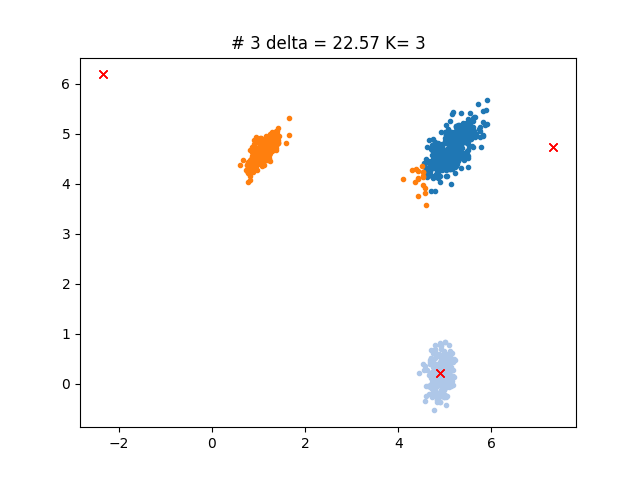
\includegraphics[width=0.33\textwidth]{20-3}
                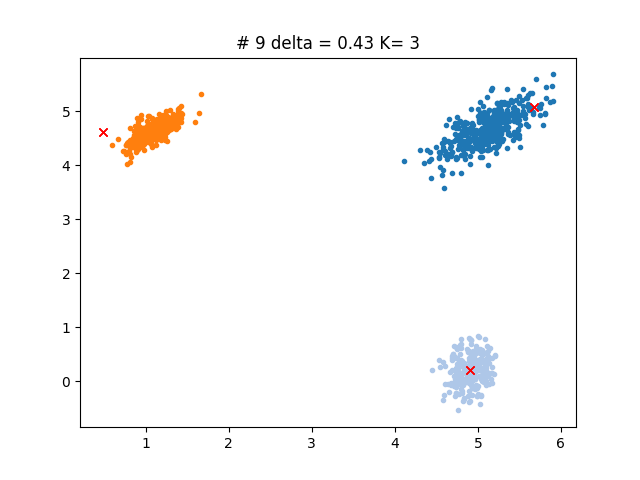
\includegraphics[width=0.33\textwidth]{20-9}
                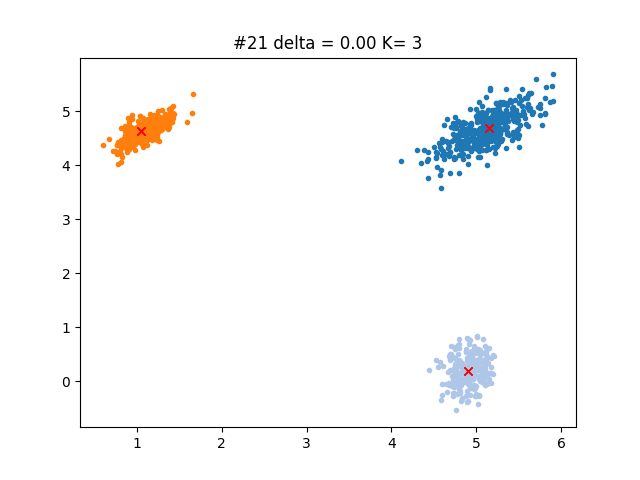
\includegraphics[width=0.33\textwidth]{20-21}
            }
            \subfigure[$K=12, \gamma=0.05$]{\label{fig:10}
                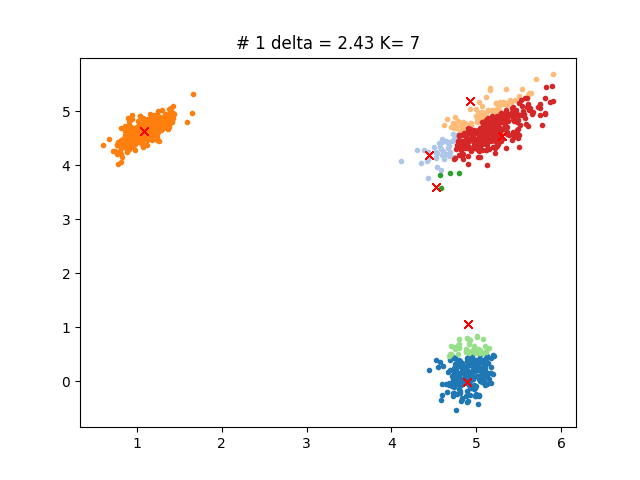
\includegraphics[width=0.33\textwidth]{10-1}
                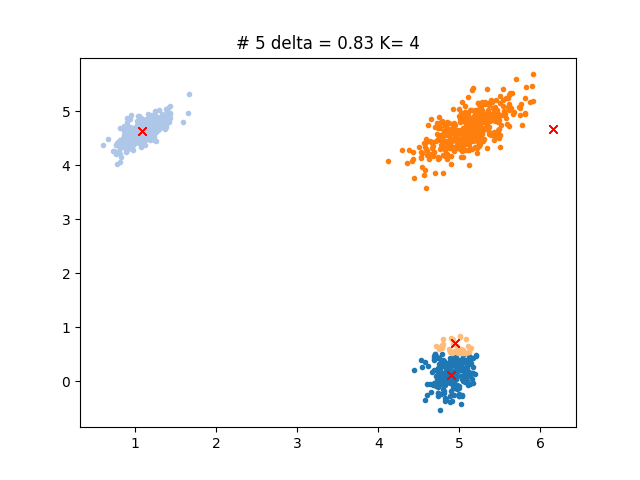
\includegraphics[width=0.33\textwidth]{10-5}
                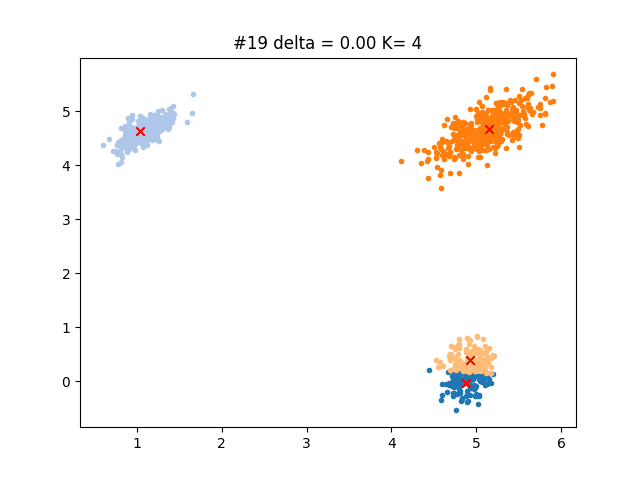
\includegraphics[width=0.33\textwidth]{10-19}
            }
            \subfigure[$K=12, \gamma=0.1$]{\label{fig:30}
                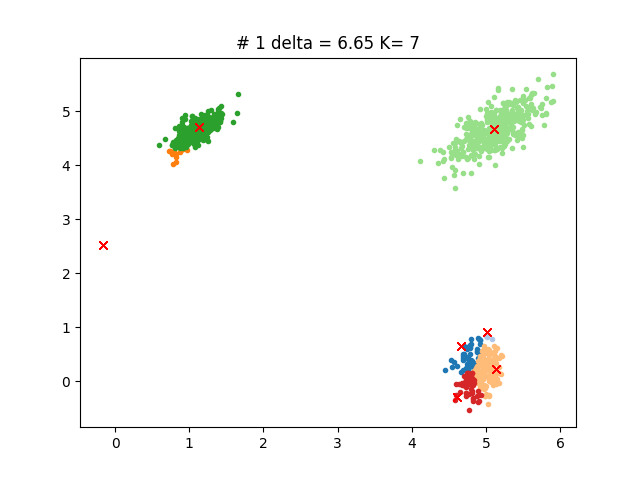
\includegraphics[width=0.33\textwidth]{30-1}
                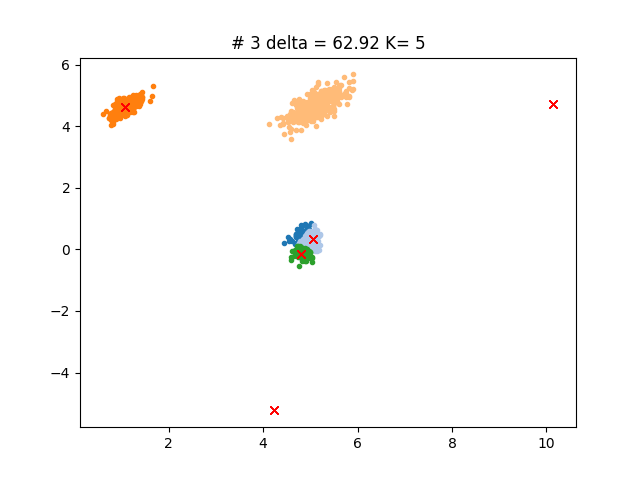
\includegraphics[width=0.33\textwidth]{30-3}
                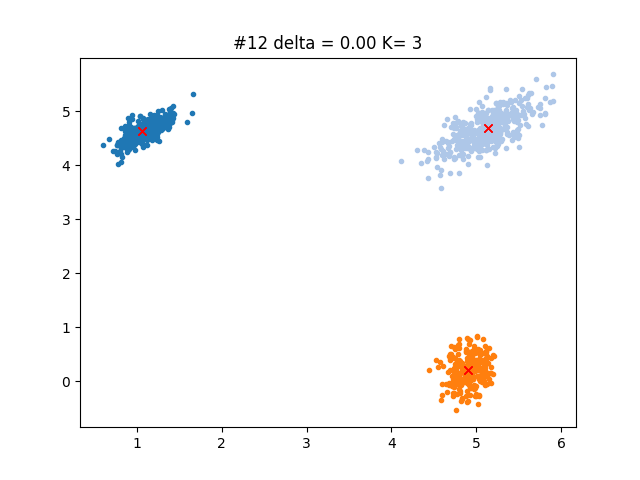
\includegraphics[width=0.33\textwidth]{30-12}
            }
            \caption{RPCL 版本的 k-mean 算法训练结果}
        \end{figure}

    \section{GMM 模型选择}

    \subsection{生成 GMM 数据}\label{sec:datagen}

    对于 $L$ 维、$K$ 个子模型的高斯混合模型(GMM),其概率密度函数定义为
    \begin{equation}
        p(\bm{x}) = \sum_{k=1}^K w_k \mathcal{N}(\bm{x}|\bm{\mu}_k,\bm{\Sigma}_k)
    \end{equation}
    其中
    \begin{equation}\label{eq:weight}
        \sum_{k=1}^K w_k = 1
    \end{equation}

    算法 \ref{alg:gmmgen} 展示了通过随机化参量、多项分布获得每个子模型的样本数、多维高斯分布采样得到 GMM 的过程\cite{gmmgen}。生成数据代码见 \filelink{src/datagen.py}。

    \begin{algorithm}
        \caption{生成 GMM 数据}\label{alg:gmmgen}
        如果指定随机种子,则初始化随机种子\;
        随机生成权重 $w_k$,归一化以满足公式 \eqref{eq:weight} 中的条件\;
        借助 \verb"numpy" 库生成随机的 $K$ 个 $L\times (K+1)$ 矩阵,计算协方差矩阵作为 GMM 数据的随机参量 $\bm{\Sigma}_k$(这一步主要为了保证协方差矩阵的对称正定\cite{multinorm}),对于均值 $\bm{\mu}_k$ 直接随机坐标并扩大 $2K$ 倍以保持一定的距离\;
        通过多项分布得到每个子模型的样本数 $N_k$\;
        对每个子模型通过多维高斯模型采样对应的样本数次数,合并得到全部的样本\;
    \end{algorithm}

    \subsection{AIC 和 BIC}

    首先计算出所有聚类数目取值 $k$ 下的模型,按照公式 \eqref{eq:kmax} 通过 AIC \eqref{eq:aic} 或 BIC \eqref{eq:bic} 的标准筛选最优聚类数目。采用 sklearn 的 \verb"sklearn.mixture.GaussianMixture" 实现 GMM 模型\cite{skgmm}。

    \begin{align}
        k^* &= {\arg\max}_{k=1,\cdots,K}J(k) \label{eq:kmax}\\
        J_\text{AIC}(k) &= \ln[p(X|\hat{\Theta}_k)] - d_m \label{eq:aic}\\
        J_\text{BIC}(k) &= \ln[p(X|\hat{\Theta}_k)] - \frac{\ln N}{2}d_m \label{eq:bic} 
    \end{align}

    对每一个二元组 (目标聚类数目, 样本数量) 采用不同的随机种子分别对 AIC 和 BIC 进行多轮实验,代码见 \filelink{src/em.py},参量范围如表 \ref{tab:exparam} 所示,结果如图 \ref{fig:em_result} 所示,红色曲面为 AIC 的结果,蓝色曲面为 BIC 的结果。

    \begin{figure}
        \begin{minipage}[b]{.5\linewidth}
            \centering
            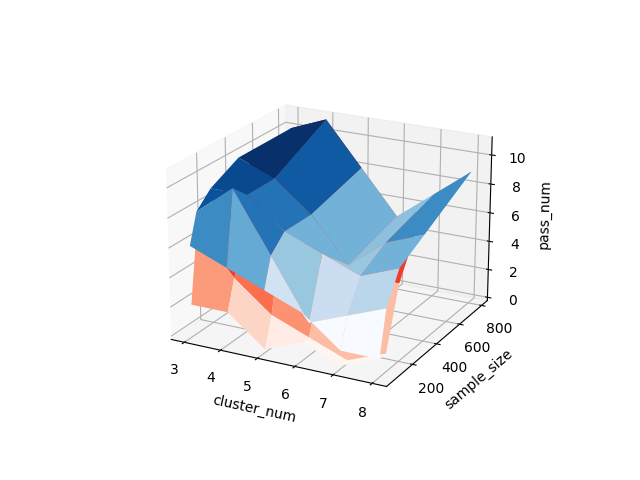
\includegraphics[width=\linewidth]{em_result.png}
            \caption{AIC (红色) 与 BIC (蓝色) 比较的实验结果}\label{fig:em_result}
        \end{minipage}
        \begin{minipage}[b]{.5\linewidth}
            \centering
            \begin{tabular}{cc}
                \toprule
                参量 & 范围 \\
                \midrule
                目标聚类数目 & (3,4,5,6,7,8) \\
                样本数量 & (50,100,200,400,800) \\
                \midrule
                随机种子 & 11 个 \\
                最大聚类数目 & 目标聚类数目 + 3 \\
                \bottomrule
            \end{tabular}
            \captionof{table}{实验参量}\label{tab:exparam}
        \end{minipage}
    \end{figure}

    对于正确率的统计表明,大部分情况下 BIC 比 AIC 的表现更好(仅有少数样本数量 $N$ 较低的时候 AIC 偶尔比 BIC 表现好一次)。当数据数量较大时这种差距不会特别明显。
    
    详细地查看错分类情形,如图 \ref{fig:false} 所示:
    \begin{enumerate}[(a)]
        \item AIC 与 BIC 均分类错误,一般由于样本量较少,目标聚类数目较大,导致有些类别的样本数量不足,且距离较近,这种情形属于数据集本身的缺陷。
        \item BIC 正确分类的时候,AIC 分类错误,这种情形 AIC 倾向于分类数目更多,这主要是由于没有被公式 \eqref{eq:aic} 中没有由样本数量 $N$ 控制,任由自由参数数量的控制的话,会导致更多的分类得到更低的得分。
        \item AIC 正确分类,BIC 分类错误,这种情形 BIC 倾向于将两个粘合的类别认为一个类别。公式 \eqref{eq:bic} 的第一项会因为更少的分类而更少,抵过了第二项的效果。
    \end{enumerate}

    \begin{figure}
        \centering
        \subfigure[AIC 与 BIC 均错误,数据集分离性差 $K=8,N=200$]{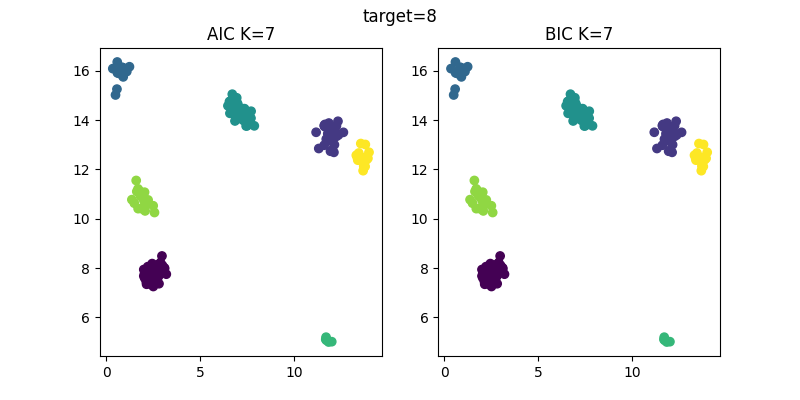
\includegraphics[width=0.8\linewidth]{em_8_200_271.png}}
        \subfigure[BIC 正确,AIC 错误地倾向于较多类别 $K=4,N=200$]{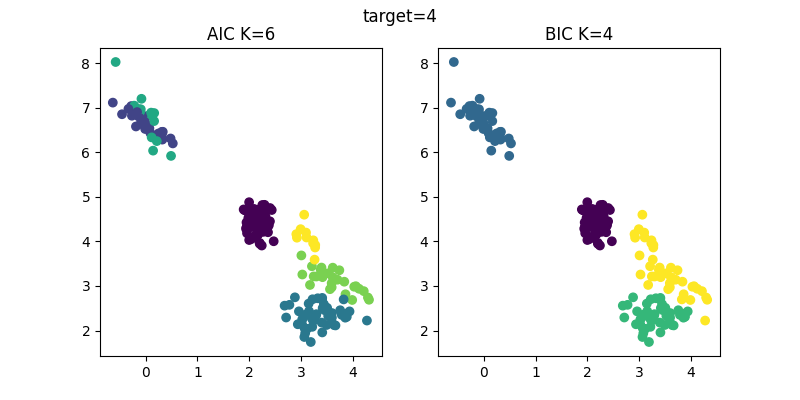
\includegraphics[width=0.8\linewidth]{em_4_200_451.png}}
        \subfigure[AIC 正确,BIC 错误地倾向于较少类别 $K=6,N=400$]{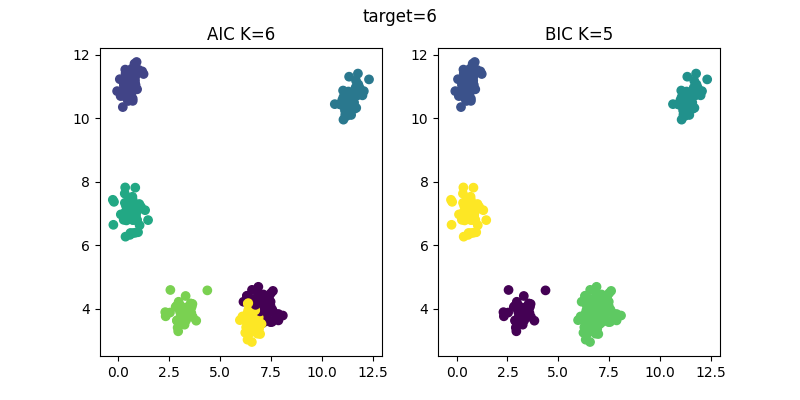
\includegraphics[width=0.8\linewidth]{em_6_400_231.png}}
        \caption{AIC 与 BIC 错分类情形}\label{fig:false}
    \end{figure}
    
    \subsection{VBEMGMM}

    VBEMGMM (Variational Bayesian estimation of a Gaussian mixture) 采用了 Bayesian 推理,遵循 Occam 准则选择最优的聚类数目。采用 sklearn 的 \verb"sklearn.mixture.BayesianGuassianMixture" 实现 VBEMGMM 模型\cite{skvbgmm}。

    向上面的测试方法中加入 VBEMGMM 的结果,正确率对比如图 \ref{fig:em_result_overall} 所示,绿色曲面代表 VBEMGMM 的结果。结果显示样本数量较少时,并不如 BIC 的分类正确率高;当样本数量变大后,与前两者的分类正确准确率基本一致。

    查看其中一个 VBEMGMM 错误分类的情形,如图 \ref{fig:vbemgmm} 所示。可以看到有一个类别由于点较少,导致可能会由于 Occam 准则被错误分类为另一组。也就意味着 VBEMGMM 对于每个聚类内样本数量较少的情况可能表现不会那么理想。

    \subsection{模型选择小结}

    当每个聚类的样本数量充足时,可以考虑使用 VBEMGMM 自动得到聚类数目,而不用跑很多次聚类过程。而当每个聚类的样本数量不充足时,如果聚类的分离比较明确,则可以使用 BIC 来得到更少的聚类数目;如果聚类有粘合时,则可以使用 AIC 来得到更多的聚类数目,获取隐性的分类信息。

    \begin{figure}
        \centering
        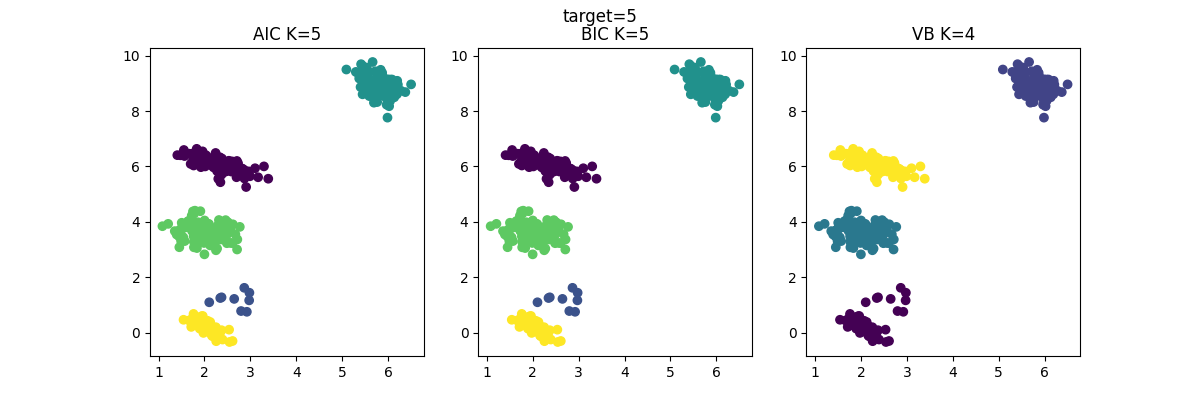
\includegraphics[width=0.8\linewidth]{em_5_400_401.png}
        \caption{VBEMGMM 分类错误情形 $K=5,N=400$}\label{fig:vbemgmm}
    \end{figure}

    \begin{figure}
        \begin{minipage}[b]{.5\linewidth}
            \centering
            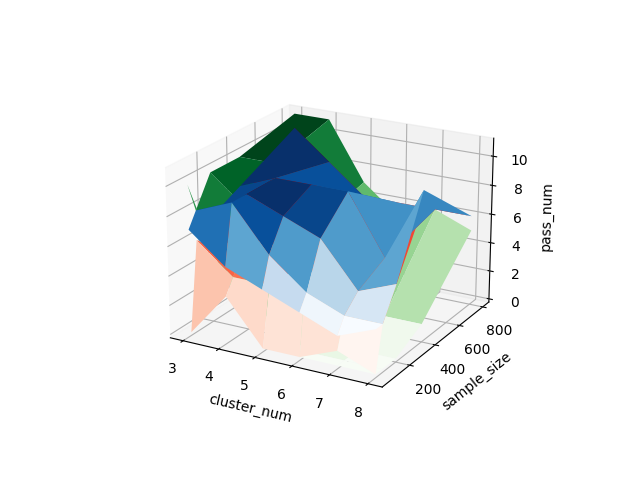
\includegraphics[width=\linewidth]{em_result_overall.png}
            \caption{AIC (红色), BIC (蓝色), VBEMGMM (绿色) 的正确分类情况曲面图}\label{fig:em_result_overall}
        \end{minipage}
        \begin{minipage}[b]{.5\linewidth}
            \centering
            \captionof{table}{AIC, BIC, VBEMGMM 的正确分类情况表,随机种子数为 11}\label{tab:em_result}
            \pgfplotstabletypeset{img/em_result.dat}
        \end{minipage}
    \end{figure}

    \clearpage

    \bibliography{ref}
\end{document}